\chapter{Desenvolvimento\label{ch:develop}}

%\begin{flushright}
%\textit{Simple, clear purpose and principles give rise to complex, intelligent behavior. Complex rules and regulations give rise to simple and stupid behavior.}\\(Hock Dee)
%\end{flushright}

Em trabalhos anteriores foram propostos e implementados vários controladores cinemáticos como forma de corrigir o efeito das pertubações devido a interação com uma agente externo e da ação da gravidade. No entanto o desempenho foi abaixo do apresentado pela código de demonstração do fabricante para o robô e pelos mesmos controladores no uso em outra plataforma explicitando a necessidade de um maior estudo da arquitetura do manipulador robótico Meka A2. Com base nisto foi feito uma análise do componentes do braço e a implementação dos sistemas de controle das juntas em software e hardware. Neste capítulo será descrito os métodos de investigação utilizados bem como experimentos efetuados.

\section{Avaliação de Desempenho}

Em \cite{nocite} Marcos propôs diversas métricas e avaliar os controladores cinemáticos implementados. Enquanto foi possível um excelente detalhamento da desempenho comparativa de cada um dos controladores, foi descoberto limitações na interação com a plataforma. Neste trabalho será analisado o robô enquanto sistema observando as implicações dos componentes mecânicos, software e sistemas de controle operando de forma conjunta. O objetivo é avaliar dentro do que já foi implementado os limites de desempenho permitidos pela plataforma para permitir um melhor desempenho em trabalhos futuros. 

% Gráfico Desempenho

Por se tratar de um sistema mecatrônico, naturalmente existem 3 camadas: Sistema Mecânico, Sistema Embarcado e Algorítimos de Controle. Para o Meka estes estão implementados na seguinte forma

\begin{itemize}
    \item Sistema Mecânico ( Atuadores Série Elásticos )
    \begin{itemize}
        \item Motores Brushless
        \item Harmonic Drive
    \end{itemize}
    \item Sistema Embarcado ( Atuadores Série Elásticos )
    \begin{itemize}
        \item Placa DSP para controle dos motores
        \item Hub EtherCAT
        \item Interface EtherCAT para o computador
        \item PC com Linux Ubuntu 12.04 e Kernel RTOS Xenomai
    \end{itemize}
    \item Algoritmos de Controle
    \begin{itemize}
        \item Controle de Torque (DSP)
        \item Controle de Posição com Compensação da Gravidade (PC)
        \item Interface ROS
        \item Controle Cinemático
        \item Gerador de Trajetória
    \end{itemize}
\end{itemize}

% Comentar sobre desempenho de sistemas
% - Como alcançar o maior desempenho do sistema ( Custo exponencial 99.9 )
% - Não linearidades identificadas

% Avaliação Sistema Mecânico
% - Estudo SEA
% - Documentação
% Avaliação Sistema Embarcado?
% - Documentação EtherCAT, RTOS, PC
% - Tempo de Resposta da Comunicação
% Avaliação Controle
% - Ensaios Estabilidade em Malha Fechada
% - Ensaios em Degrau

% TODO Colocar nos resultados:
%No qual foi observado que aspectos particulares da plataforma não foram levados em conta como a operação em regiões não lineares do sistema devido a saturação da velocidade e torque dos motores, tempos longo de atraso de comunicação entre o computador.

% Reprodução Resultados Marcos

\section{Avaliação Preliminar}

Inicialmente foi feito um estudo a partir do código de demonstração do fabricante feito em Python para avaliar quais as possíveis forma de controlar o braço. Em que foi levantando todos os controladores implementados na biblioteca m3 e testados individualmente através da API em Python. Estão disponíveis os seguintes controladores pela biblioteca:

\begin{itemize}
    \item Controle de Posição
    \item Controle de Posição com compensação da gravidade
    \item Controle de Torque
    \item Controle de Torque com compensação da gravidade
    \item Controle de Velocidade
\end{itemize}

%Nesta avaliação foi notado que alguns dos controladores da m3 não estavam disponíveis nas interfaces em C++. 

Para análise do comportamento em conjunto dos controladores cinemáticos foi definido o controlador de posição com compensação da gravidade, uma vez que este que é usado pela ROS.

\section{Estudo Controladores Cinemáticos}

Para definir um ponto de referência para os ensaios e testes, foram avaliados os controladores implementados por Marcos Pereira. A partir da melhor configuração para cada um dos controladores foram feitos experimentos ajustando os parâmetros da velocidade de atuação e nível rigidez para avaliar a influência nos resultados. Os experimentos foram executados foram feitos com base em duas trajetórias pré-definidas: deslocamento em linha reta na vertical e o desenho de um quadrado a partir de dois deslocamentos na vertical e dois na horizontal.

Nos experimentos de deslocamento em linha reta foram avaliados o intervalo de tempo até robô começar a responder e o controle estabilizar para diferentes taxas de amostragem da trajetória. Enquanto nos experimentos com a trajetória de quadrado foram avaliadas a resposta do robô para diferentes valores de ajuste dos controladores de junta quanto aos parâmetros de velocidade e rigidez.

\subsection{Avaliação tempo de amostragem}

Para avaliar os tempos de atuação foi repetido o mesmo experimento para o deslocamento em linha reta na vertical. Neste experimento foi estudado o tempo necessário para o atuador começar a se mover dado um comando bem o tempo necessário para o controle convergir.

% Resultados

\subsection{Estudo Interação do controle de rigidez}

\section{Identificação}

Para avaliar a resposta do sistema para controle dos ângulos de junta foi proposto um teste com estímulo pelo degrau. Esta avaliação foi efetuada para interação pela API em Python e pelo ROS. Para ambos casos os dados obtidos foram registrados em arquivo utilizando a ferramenta rosbag. 

% Comentar sobre como a informação é publicada nos tópicos

% Levantamento dos problemas

% Investigação de possíveis causas

\section{Meka PC}

Para o controle do robô é utilizado um computador embarcado com o sistema operacional Ubuntu 12.04 e o Kernel Real Time Xenomai. Nele são implementado o driver para o protocolo EtherCAT e a biblioteca M3 responsável pela interação com cada um dos dispositivos, entre sensores e motores de cada junta.

Dentro do pc é executado um script que para disparar os processos relacionados a comunicação com a robô via socket pelo protocolo Ethercat e as interface para Python. Um vez que o script está em execução o robô pode ser controlado via API ou por meio de um programa para ROS, conforme ilustrado no diagrama apresentado na figura \ref{fig:m3arch}.

% m3rt_server
% -> Interface via socket
% -> Memórica compartilhada
% -> API Python
% -> ROS

\begin{figure}[ht]
    \centering
    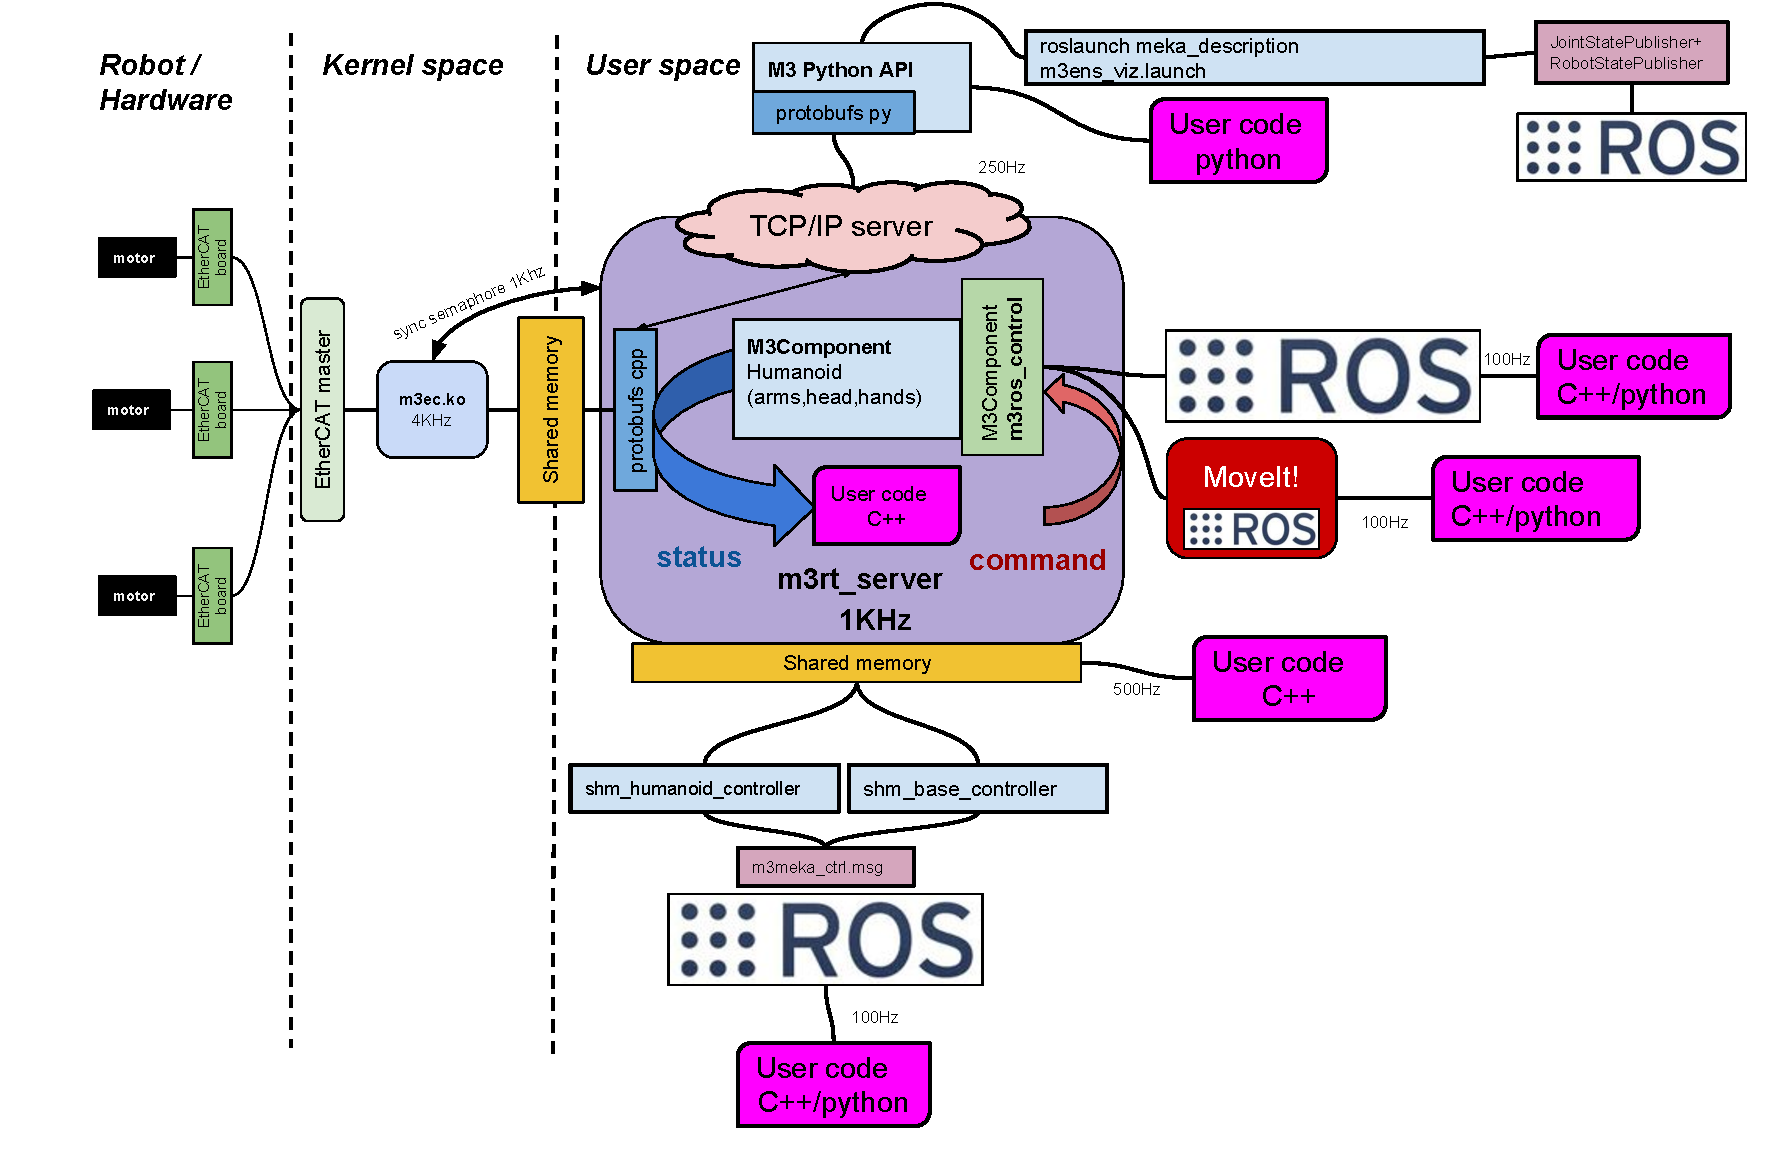
\includegraphics[width=\linewidth]{figs/m3_arch.pdf}
    \caption{Diagrama da arquitetura do robô\cite{nobody}}
    \label{fig:m3arch}
\end{figure}

